% Options for packages loaded elsewhere
\PassOptionsToPackage{unicode}{hyperref}
\PassOptionsToPackage{hyphens}{url}
%
\documentclass[
]{article}
\usepackage{amsmath,amssymb}
\usepackage{lmodern}
\usepackage{iftex}
\ifPDFTeX
  \usepackage[T1]{fontenc}
  \usepackage[utf8]{inputenc}
  \usepackage{textcomp} % provide euro and other symbols
\else % if luatex or xetex
  \usepackage{unicode-math}
  \defaultfontfeatures{Scale=MatchLowercase}
  \defaultfontfeatures[\rmfamily]{Ligatures=TeX,Scale=1}
\fi
% Use upquote if available, for straight quotes in verbatim environments
\IfFileExists{upquote.sty}{\usepackage{upquote}}{}
\IfFileExists{microtype.sty}{% use microtype if available
  \usepackage[]{microtype}
  \UseMicrotypeSet[protrusion]{basicmath} % disable protrusion for tt fonts
}{}
\makeatletter
\@ifundefined{KOMAClassName}{% if non-KOMA class
  \IfFileExists{parskip.sty}{%
    \usepackage{parskip}
  }{% else
    \setlength{\parindent}{0pt}
    \setlength{\parskip}{6pt plus 2pt minus 1pt}}
}{% if KOMA class
  \KOMAoptions{parskip=half}}
\makeatother
\usepackage{xcolor}
\usepackage[margin=1in]{geometry}
\usepackage{color}
\usepackage{fancyvrb}
\newcommand{\VerbBar}{|}
\newcommand{\VERB}{\Verb[commandchars=\\\{\}]}
\DefineVerbatimEnvironment{Highlighting}{Verbatim}{commandchars=\\\{\}}
% Add ',fontsize=\small' for more characters per line
\usepackage{framed}
\definecolor{shadecolor}{RGB}{248,248,248}
\newenvironment{Shaded}{\begin{snugshade}}{\end{snugshade}}
\newcommand{\AlertTok}[1]{\textcolor[rgb]{0.94,0.16,0.16}{#1}}
\newcommand{\AnnotationTok}[1]{\textcolor[rgb]{0.56,0.35,0.01}{\textbf{\textit{#1}}}}
\newcommand{\AttributeTok}[1]{\textcolor[rgb]{0.77,0.63,0.00}{#1}}
\newcommand{\BaseNTok}[1]{\textcolor[rgb]{0.00,0.00,0.81}{#1}}
\newcommand{\BuiltInTok}[1]{#1}
\newcommand{\CharTok}[1]{\textcolor[rgb]{0.31,0.60,0.02}{#1}}
\newcommand{\CommentTok}[1]{\textcolor[rgb]{0.56,0.35,0.01}{\textit{#1}}}
\newcommand{\CommentVarTok}[1]{\textcolor[rgb]{0.56,0.35,0.01}{\textbf{\textit{#1}}}}
\newcommand{\ConstantTok}[1]{\textcolor[rgb]{0.00,0.00,0.00}{#1}}
\newcommand{\ControlFlowTok}[1]{\textcolor[rgb]{0.13,0.29,0.53}{\textbf{#1}}}
\newcommand{\DataTypeTok}[1]{\textcolor[rgb]{0.13,0.29,0.53}{#1}}
\newcommand{\DecValTok}[1]{\textcolor[rgb]{0.00,0.00,0.81}{#1}}
\newcommand{\DocumentationTok}[1]{\textcolor[rgb]{0.56,0.35,0.01}{\textbf{\textit{#1}}}}
\newcommand{\ErrorTok}[1]{\textcolor[rgb]{0.64,0.00,0.00}{\textbf{#1}}}
\newcommand{\ExtensionTok}[1]{#1}
\newcommand{\FloatTok}[1]{\textcolor[rgb]{0.00,0.00,0.81}{#1}}
\newcommand{\FunctionTok}[1]{\textcolor[rgb]{0.00,0.00,0.00}{#1}}
\newcommand{\ImportTok}[1]{#1}
\newcommand{\InformationTok}[1]{\textcolor[rgb]{0.56,0.35,0.01}{\textbf{\textit{#1}}}}
\newcommand{\KeywordTok}[1]{\textcolor[rgb]{0.13,0.29,0.53}{\textbf{#1}}}
\newcommand{\NormalTok}[1]{#1}
\newcommand{\OperatorTok}[1]{\textcolor[rgb]{0.81,0.36,0.00}{\textbf{#1}}}
\newcommand{\OtherTok}[1]{\textcolor[rgb]{0.56,0.35,0.01}{#1}}
\newcommand{\PreprocessorTok}[1]{\textcolor[rgb]{0.56,0.35,0.01}{\textit{#1}}}
\newcommand{\RegionMarkerTok}[1]{#1}
\newcommand{\SpecialCharTok}[1]{\textcolor[rgb]{0.00,0.00,0.00}{#1}}
\newcommand{\SpecialStringTok}[1]{\textcolor[rgb]{0.31,0.60,0.02}{#1}}
\newcommand{\StringTok}[1]{\textcolor[rgb]{0.31,0.60,0.02}{#1}}
\newcommand{\VariableTok}[1]{\textcolor[rgb]{0.00,0.00,0.00}{#1}}
\newcommand{\VerbatimStringTok}[1]{\textcolor[rgb]{0.31,0.60,0.02}{#1}}
\newcommand{\WarningTok}[1]{\textcolor[rgb]{0.56,0.35,0.01}{\textbf{\textit{#1}}}}
\usepackage{graphicx}
\makeatletter
\def\maxwidth{\ifdim\Gin@nat@width>\linewidth\linewidth\else\Gin@nat@width\fi}
\def\maxheight{\ifdim\Gin@nat@height>\textheight\textheight\else\Gin@nat@height\fi}
\makeatother
% Scale images if necessary, so that they will not overflow the page
% margins by default, and it is still possible to overwrite the defaults
% using explicit options in \includegraphics[width, height, ...]{}
\setkeys{Gin}{width=\maxwidth,height=\maxheight,keepaspectratio}
% Set default figure placement to htbp
\makeatletter
\def\fps@figure{htbp}
\makeatother
\setlength{\emergencystretch}{3em} % prevent overfull lines
\providecommand{\tightlist}{%
  \setlength{\itemsep}{0pt}\setlength{\parskip}{0pt}}
\setcounter{secnumdepth}{-\maxdimen} % remove section numbering
\ifLuaTeX
  \usepackage{selnolig}  % disable illegal ligatures
\fi
\IfFileExists{bookmark.sty}{\usepackage{bookmark}}{\usepackage{hyperref}}
\IfFileExists{xurl.sty}{\usepackage{xurl}}{} % add URL line breaks if available
\urlstyle{same} % disable monospaced font for URLs
\hypersetup{
  pdftitle={Practica\_2},
  pdfauthor={Felipe Vásquez},
  hidelinks,
  pdfcreator={LaTeX via pandoc}}

\title{Practica\_2}
\author{Felipe Vásquez}
\date{2023-04-23}

\begin{document}
\maketitle

{
\setcounter{tocdepth}{2}
\tableofcontents
}
\hypertarget{pregunta-1}{%
\subsubsection{Pregunta 1}\label{pregunta-1}}

1. Descargar la página web de la URL indicada, y almacenarlo en un
formato de R apto para ser tratado.

\begin{Shaded}
\begin{Highlighting}[]
\CommentTok{\#URL}
\NormalTok{url }\OtherTok{\textless{}{-}} \StringTok{"https://www.mediawiki.org/wiki/MediaWiki"}
\CommentTok{\#Download page}
\NormalTok{page }\OtherTok{\textless{}{-}} \FunctionTok{GET}\NormalTok{(url)}
\CommentTok{\#Status}
\FunctionTok{status\_code}\NormalTok{(page)}
\end{Highlighting}
\end{Shaded}

\begin{verbatim}
## [1] 200
\end{verbatim}

\begin{Shaded}
\begin{Highlighting}[]
\CommentTok{\#De HTML a formato XML}
\NormalTok{parsed\_page }\OtherTok{\textless{}{-}} \FunctionTok{htmlParse}\NormalTok{(}\FunctionTok{content}\NormalTok{(page, }\AttributeTok{as =} \StringTok{"text"}\NormalTok{))}
\end{Highlighting}
\end{Shaded}

2. Analizar el contenido de la web, buscando el título de la página (que
en HTML se etiqueta como ``title'').

\begin{Shaded}
\begin{Highlighting}[]
\CommentTok{\#Título pagina}
\NormalTok{title }\OtherTok{\textless{}{-}} \FunctionTok{xpathSApply}\NormalTok{(parsed\_page, }\StringTok{"//title"}\NormalTok{, xmlValue)}
\NormalTok{title}
\end{Highlighting}
\end{Shaded}

\begin{verbatim}
## [1] "MediaWiki"
\end{verbatim}

\begin{Shaded}
\begin{Highlighting}[]
\CommentTok{\#Styless}
\NormalTok{stylesheets }\OtherTok{\textless{}{-}} \FunctionTok{xpathSApply}\NormalTok{(parsed\_page, }\StringTok{"//link[@rel=\textquotesingle{}stylesheet\textquotesingle{}]/@href"}\NormalTok{)}
\NormalTok{stylesheets}
\end{Highlighting}
\end{Shaded}

\begin{verbatim}
##                                                                                                                                                                                                                                                                                                                           href 
## "/w/load.php?lang=en&modules=ext.discussionTools.init.styles%7Cext.uls.pt%7Cext.visualEditor.desktopArticleTarget.noscript%7Cext.wikimediaBadges%7Cmediawiki.ui.button%2Cicon%7Cmediawiki.widgets.styles%7Coojs-ui-core.icons%2Cstyles%7Coojs-ui.styles.indicators%7Cskins.vector.icons%2Cstyles&only=styles&skin=vector-2022" 
##                                                                                                                                                                                                                                                                                                                           href 
##                                                                                                                                                                                                                                              "/w/load.php?lang=en&modules=ext.gadget.site-styles&only=styles&skin=vector-2022" 
##                                                                                                                                                                                                                                                                                                                           href 
##                                                                                                                                                                                                                                                         "/w/load.php?lang=en&modules=site.styles&only=styles&skin=vector-2022"
\end{verbatim}

\begin{Shaded}
\begin{Highlighting}[]
\CommentTok{\#Autor}
\NormalTok{author }\OtherTok{\textless{}{-}} \FunctionTok{xpathSApply}\NormalTok{(parsed\_page, }\StringTok{"//meta[@name=\textquotesingle{}author\textquotesingle{}]/@content"}\NormalTok{)}
\NormalTok{author}
\end{Highlighting}
\end{Shaded}

\begin{verbatim}
## NULL
\end{verbatim}

\begin{Shaded}
\begin{Highlighting}[]
\CommentTok{\#Descripcion}
\NormalTok{description }\OtherTok{\textless{}{-}} \FunctionTok{xpathSApply}\NormalTok{(parsed\_page, }\StringTok{"//meta[@name=\textquotesingle{}description\textquotesingle{}]/@content"}\NormalTok{)}
\NormalTok{description}
\end{Highlighting}
\end{Shaded}

\begin{verbatim}
## NULL
\end{verbatim}

\begin{Shaded}
\begin{Highlighting}[]
\CommentTok{\#Codificación Type}
\NormalTok{encoding }\OtherTok{\textless{}{-}} \FunctionTok{xpathSApply}\NormalTok{(parsed\_page, }\StringTok{"//meta[@charset]/@charset"}\NormalTok{)}
\NormalTok{encoding}
\end{Highlighting}
\end{Shaded}

\begin{verbatim}
## charset 
## "UTF-8"
\end{verbatim}

\begin{Shaded}
\begin{Highlighting}[]
\CommentTok{\#keywords}
\NormalTok{keywords }\OtherTok{\textless{}{-}} \FunctionTok{xpathSApply}\NormalTok{(parsed\_page, }\StringTok{"//meta[@name=\textquotesingle{}keywords\textquotesingle{}]/@content"}\NormalTok{)}
\NormalTok{keywords}
\end{Highlighting}
\end{Shaded}

\begin{verbatim}
## NULL
\end{verbatim}

3. Analizar el contenido de la web, buscando todos los enlaces (que en
HTML se etiquetan como ``a''), buscando el texto del enlace, así como la
URL.

\begin{Shaded}
\begin{Highlighting}[]
\CommentTok{\#Texto del enlace}
\NormalTok{links\_text }\OtherTok{\textless{}{-}} \FunctionTok{xpathSApply}\NormalTok{(parsed\_page, }\StringTok{"//a"}\NormalTok{, xmlValue)}
\FunctionTok{print}\NormalTok{(links\_text)}
\end{Highlighting}
\end{Shaded}

\begin{verbatim}
##   [1] "Jump to content"                                                    
##   [2] "Main page"                                                          
##   [3] "Get MediaWiki"                                                      
##   [4] "Get extensions"                                                     
##   [5] "Tech blog"                                                          
##   [6] "Contribute"                                                         
##   [7] "User help"                                                          
##   [8] "FAQ"                                                                
##   [9] "Technical manual"                                                   
##  [10] "Support desk"                                                       
##  [11] "Communication"                                                      
##  [12] "Developer portal"                                                   
##  [13] "Code statistics"                                                    
##  [14] "Community portal"                                                   
##  [15] "Recent changes"                                                     
##  [16] "Translate content"                                                  
##  [17] "Random page"                                                        
##  [18] "Village pump"                                                       
##  [19] "Sandbox"                                                            
##  [20] "\n\t\n\t\t\n"                                                       
##  [21] "\n\t\tSearch\n\t"                                                   
##  [22] " English"                                                           
##  [23] "Create account"                                                     
##  [24] "Log in"                                                             
##  [25] " Create account"                                                    
##  [26] " Log in"                                                            
##  [27] "learn more"                                                         
##  [28] "Contributions"                                                      
##  [29] "Talk"                                                               
##  [30] "Main Page"                                                          
##  [31] "Discussion"                                                         
##  [32] "Read"                                                               
##  [33] "View source"                                                        
##  [34] "View history"                                                       
##  [35] "Read"                                                               
##  [36] "View source"                                                        
##  [37] "View history"                                                       
##  [38] "What links here"                                                    
##  [39] "Related changes"                                                    
##  [40] "Upload file"                                                        
##  [41] "Special pages"                                                      
##  [42] "Permanent link"                                                     
##  [43] "Page information"                                                   
##  [44] "Cite this page"                                                     
##  [45] "Wikidata item"                                                      
##  [46] "Create a book"                                                      
##  [47] "Download as PDF"                                                    
##  [48] "Printable version"                                                  
##  [49] "Wikimedia Commons"                                                  
##  [50] "Meta-Wiki"                                                          
##  [51] "Multilingual Wikisource"                                            
##  [52] "Wikispecies"                                                        
##  [53] "Wikibooks"                                                          
##  [54] "Wikidata"                                                           
##  [55] "Wikimania"                                                          
##  [56] "Wikinews"                                                           
##  [57] "Wikipedia"                                                          
##  [58] "Wikiquote"                                                          
##  [59] "Wikisource"                                                         
##  [60] "Wikiversity"                                                        
##  [61] "Wikivoyage"                                                         
##  [62] "Wiktionary"                                                         
##  [63] ""                                                                   
##  [64] "tens of thousands of websites"                                      
##  [65] "thousands of companies and organizations"                           
##  [66] "multilingual"                                                       
##  [67] "free and open"                                                      
##  [68] "Find out more"                                                      
##  [69] "if MediaWiki is right for you"                                      
##  [70] "Download"                                                           
##  [71] "install"                                                            
##  [72] "configure"                                                          
##  [73] "extensions"                                                         
##  [74] "errors and symptoms"                                                
##  [75] "FAQ"                                                                
##  [76] "hosting services"                                                   
##  [77] "Get professional development and consulting"                        
##  [78] " "                                                                  
##  [79] "MediaWiki Stakeholders"                                             
##  [80] "Learn how to navigate"                                              
##  [81] " "                                                                  
##  [82] "Learn how to edit a page"                                           
##  [83] " "                                                                  
##  [84] "Learn more about reading, editing, and personal customization"      
##  [85] " "                                                                  
##  [86] "developer documentation"                                            
##  [87] "Wikimedia Developer Portal"                                         
##  [88] "support desk"                                                       
##  [89] "Get involved"                                                       
##  [90] "Report wrong software behavior or a feature proposal"               
##  [91] " "                                                                  
##  [92] "MediaWiki 1.35.10, 1.38.6 and 1.39.3 security releases"             
##  [93] "EMWCon"                                                             
##  [94] "View livestream"                                                    
##  [95] "Wikimedia Hackathon"                                                
##  [96] "@mediawiki@wikis.world"                                             
##  [97] "More news"                                                          
##  [98] "Other languages:"                                                   
##  [99] " "                                                                  
## [100] "English"                                                            
## [101] "Afrikaans"                                                          
## [102] "العربية"                                                            
## [103] "asturianu"                                                          
## [104] "беларуская"                                                         
## [105] "беларуская (тарашкевіца)"                                           
## [106] "български"                                                          
## [107] "বাংলা"                                                              
## [108] "bosanski"                                                           
## [109] "català"                                                             
## [110] "کوردی"                                                              
## [111] "čeština"                                                            
## [112] "dansk"                                                              
## [113] "Deutsch"                                                            
## [114] "español"                                                            
## [115] "فارسی"                                                              
## [116] "suomi"                                                              
## [117] "français"                                                           
## [118] "ગુજરાતી"                                                             
## [119] "עברית"                                                              
## [120] "हिन्दी"                                                              
## [121] "hrvatski"                                                           
## [122] "magyar"                                                             
## [123] "հայերեն"                                                            
## [124] "Bahasa Indonesia"                                                   
## [125] "italiano"                                                           
## [126] "日本語"                                                             
## [127] "Jawa"                                                               
## [128] "қазақша"                                                            
## [129] "한국어"                                                             
## [130] "Bahasa Melayu"                                                      
## [131] "Mirandés"                                                           
## [132] "Nederlands"                                                         
## [133] "polski"                                                             
## [134] "português"                                                          
## [135] "português do Brasil"                                                
## [136] "română"                                                             
## [137] "русский"                                                            
## [138] "sardu"                                                              
## [139] "සිංහල"                                                               
## [140] "slovenčina"                                                         
## [141] "slovenščina"                                                        
## [142] "Soomaaliga"                                                         
## [143] "shqip"                                                              
## [144] "српски / srpski"                                                    
## [145] "svenska"                                                            
## [146] "ไทย"                                                                
## [147] "Türkçe"                                                             
## [148] "українська"                                                         
## [149] "Tiếng Việt"                                                         
## [150] "粵語"                                                               
## [151] "中文"                                                               
## [152] "https://www.mediawiki.org/w/index.php?title=MediaWiki&oldid=3878227"
## [153] "Languages pages"                                                    
## [154] "Creative Commons Attribution-ShareAlike License"                    
## [155] "Terms of Use"                                                       
## [156] "Privacy policy"                                                     
## [157] "About MediaWiki.org"                                                
## [158] "Disclaimers"                                                        
## [159] "Code of Conduct"                                                    
## [160] "Mobile view"                                                        
## [161] "Developers"                                                         
## [162] "Statistics"                                                         
## [163] "Cookie statement"                                                   
## [164] ""                                                                   
## [165] ""
\end{verbatim}

\begin{Shaded}
\begin{Highlighting}[]
\CommentTok{\#URL}
\NormalTok{links\_url }\OtherTok{\textless{}{-}} \FunctionTok{xpathSApply}\NormalTok{(parsed\_page, }\StringTok{"//a"}\NormalTok{, xmlGetAttr, }\StringTok{\textquotesingle{}href\textquotesingle{}}\NormalTok{)}
\FunctionTok{print}\NormalTok{(links\_url)}
\end{Highlighting}
\end{Shaded}

\begin{verbatim}
##   [1] "#bodyContent"                                                                                                                
##   [2] "/wiki/MediaWiki"                                                                                                             
##   [3] "/wiki/Download"                                                                                                              
##   [4] "/wiki/Special:MyLanguage/Category:Extensions"                                                                                
##   [5] "//techblog.wikimedia.org/"                                                                                                   
##   [6] "/wiki/Special:MyLanguage/How_to_contribute"                                                                                  
##   [7] "/wiki/Special:MyLanguage/Help:Contents"                                                                                      
##   [8] "/wiki/Special:MyLanguage/Manual:FAQ"                                                                                         
##   [9] "/wiki/Special:MyLanguage/Manual:Contents"                                                                                    
##  [10] "/wiki/Project:Support_desk"                                                                                                  
##  [11] "/wiki/Special:MyLanguage/Communication"                                                                                      
##  [12] "https://developer.wikimedia.org/"                                                                                            
##  [13] "/wiki/Development_statistics"                                                                                                
##  [14] "/wiki/Project:Help"                                                                                                          
##  [15] "/wiki/Special:RecentChanges"                                                                                                 
##  [16] "/wiki/Special:LanguageStats"                                                                                                 
##  [17] "/wiki/Special:Random"                                                                                                        
##  [18] "/wiki/Project:Village_Pump"                                                                                                  
##  [19] "/wiki/Project:Sandbox"                                                                                                       
##  [20] "/wiki/MediaWiki"                                                                                                             
##  [21] "/wiki/Special:Search"                                                                                                        
##  [22] "#"                                                                                                                           
##  [23] "/w/index.php?title=Special:CreateAccount&returnto=MediaWiki"                                                                 
##  [24] "/w/index.php?title=Special:UserLogin&returnto=MediaWiki"                                                                     
##  [25] "/w/index.php?title=Special:CreateAccount&returnto=MediaWiki"                                                                 
##  [26] "/w/index.php?title=Special:UserLogin&returnto=MediaWiki"                                                                     
##  [27] "/wiki/Help:Introduction"                                                                                                     
##  [28] "/wiki/Special:MyContributions"                                                                                               
##  [29] "/wiki/Special:MyTalk"                                                                                                        
##  [30] "/wiki/MediaWiki"                                                                                                             
##  [31] "/wiki/Talk:MediaWiki"                                                                                                        
##  [32] "/wiki/MediaWiki"                                                                                                             
##  [33] "/w/index.php?title=MediaWiki&action=edit"                                                                                    
##  [34] "/w/index.php?title=MediaWiki&action=history"                                                                                 
##  [35] "/wiki/MediaWiki"                                                                                                             
##  [36] "/w/index.php?title=MediaWiki&action=edit"                                                                                    
##  [37] "/w/index.php?title=MediaWiki&action=history"                                                                                 
##  [38] "/wiki/Special:WhatLinksHere/MediaWiki"                                                                                       
##  [39] "/wiki/Special:RecentChangesLinked/MediaWiki"                                                                                 
##  [40] "//commons.wikimedia.org/wiki/Special:UploadWizard"                                                                           
##  [41] "/wiki/Special:SpecialPages"                                                                                                  
##  [42] "/w/index.php?title=MediaWiki&oldid=3878227"                                                                                  
##  [43] "/w/index.php?title=MediaWiki&action=info"                                                                                    
##  [44] "/w/index.php?title=Special:CiteThisPage&page=MediaWiki&id=3878227&wpFormIdentifier=titleform"                                
##  [45] "https://www.wikidata.org/wiki/Special:EntityPage/Q5296"                                                                      
##  [46] "/w/index.php?title=Special:Book&bookcmd=book_creator&referer=MediaWiki"                                                      
##  [47] "/w/index.php?title=Special:DownloadAsPdf&page=MediaWiki&action=show-download-screen"                                         
##  [48] "/w/index.php?title=MediaWiki&printable=yes"                                                                                  
##  [49] "https://commons.wikimedia.org/wiki/Main_Page"                                                                                
##  [50] "https://meta.wikimedia.org/wiki/Main_Page"                                                                                   
##  [51] "https://wikisource.org/wiki/Main_Page"                                                                                       
##  [52] "https://species.wikimedia.org/wiki/Main_Page"                                                                                
##  [53] "https://en.wikibooks.org/wiki/Main_Page"                                                                                     
##  [54] "https://www.wikidata.org/wiki/Wikidata:Main_Page"                                                                            
##  [55] "https://wikimania.wikimedia.org/wiki/Wikimania"                                                                              
##  [56] "https://en.wikinews.org/wiki/Main_Page"                                                                                      
##  [57] "https://en.wikipedia.org/wiki/Main_Page"                                                                                     
##  [58] "https://en.wikiquote.org/wiki/Main_Page"                                                                                     
##  [59] "https://en.wikisource.org/wiki/Main_Page"                                                                                    
##  [60] "https://en.wikiversity.org/wiki/Wikiversity:Main_Page"                                                                       
##  [61] "https://en.wikivoyage.org/wiki/Main_Page"                                                                                    
##  [62] "https://en.wiktionary.org/wiki/Wiktionary:Main_Page"                                                                         
##  [63] "/wiki/File:Wikimedia_Hackathon_Prague_2019_-_Group_Photo_-_CLK_-_cropped.jpg"                                                
##  [64] "/wiki/Special:MyLanguage/Sites_using_MediaWiki"                                                                              
##  [65] "/wiki/Special:MyLanguage/MediaWiki_testimonials"                                                                             
##  [66] "/wiki/Special:MyLanguage/Localisation"                                                                                       
##  [67] "https://en.wikipedia.org/wiki/FLOSS"                                                                                         
##  [68] "/wiki/Special:MyLanguage/Manual:What_is_MediaWiki%3F"                                                                        
##  [69] "/wiki/Special:MyLanguage/Manual:Deciding_whether_to_use_a_wiki_as_your_website_type"                                         
##  [70] "/wiki/Special:MyLanguage/Download"                                                                                           
##  [71] "/wiki/Special:MyLanguage/Manual:Installation_guide"                                                                          
##  [72] "/wiki/Special:MyLanguage/Manual:System_administration"                                                                       
##  [73] "/wiki/Special:MyLanguage/Manual:Extensions"                                                                                  
##  [74] "/wiki/Special:MyLanguage/Manual:Errors_and_symptoms"                                                                         
##  [75] "/wiki/Special:MyLanguage/Manual:FAQ"                                                                                         
##  [76] "/wiki/Special:MyLanguage/Hosting_services"                                                                                   
##  [77] "/wiki/Special:MyLanguage/Professional_development_and_consulting"                                                            
##  [78] "/wiki/Professional_development_and_consulting"                                                                               
##  [79] "/wiki/Special:MyLanguage/MediaWiki_Stakeholders%27_Group"                                                                    
##  [80] "/wiki/Special:MyLanguage/Help:Navigation"                                                                                    
##  [81] "/wiki/Help:Navigation"                                                                                                       
##  [82] "/wiki/Special:MyLanguage/Help:Editing_pages"                                                                                 
##  [83] "/wiki/Help:Editing_pages"                                                                                                    
##  [84] "/wiki/Special:MyLanguage/Help:Contents"                                                                                      
##  [85] "/wiki/Help:Contents"                                                                                                         
##  [86] "/wiki/Special:MyLanguage/Developer_hub"                                                                                      
##  [87] "https://developer.wikimedia.org"                                                                                             
##  [88] "/wiki/Project:Support_desk"                                                                                                  
##  [89] "/wiki/Special:MyLanguage/How_to_contribute"                                                                                  
##  [90] "/wiki/Special:MyLanguage/How_to_report_a_bug"                                                                                
##  [91] "/wiki/How_to_report_a_bug"                                                                                                   
##  [92] "https://lists.wikimedia.org/hyperkitty/list/mediawiki-announce@lists.wikimedia.org/message/6UQBHI5FWLATD7QO7DI4YS54U7XSSLAN/"
##  [93] "/wiki/Special:MyLanguage/EMWCon_Spring_2023"                                                                                 
##  [94] "https://www.youtube.com/watch?v=r0xEhy9bBFU"                                                                                 
##  [95] "/wiki/Special:MyLanguage/Wikimedia_Hackathon_2023"                                                                           
##  [96] "https://wikis.world/@mediawiki"                                                                                              
##  [97] "https://www.mediawiki.org/wiki/Special:MyLanguage/News"                                                                      
##  [98] "/wiki/Special:MyLanguage/Project:Language_policy"                                                                            
##  [99] "/wiki/Project:Language_policy"                                                                                               
## [100] "/wiki/Template:Main_page"                                                                                                    
## [101] "https://www.mediawiki.org/wiki/Template:Main_page/af"                                                                        
## [102] "https://www.mediawiki.org/wiki/Template:Main_page/ar"                                                                        
## [103] "https://www.mediawiki.org/wiki/Template:Main_page/ast"                                                                       
## [104] "https://www.mediawiki.org/wiki/Template:Main_page/be"                                                                        
## [105] "https://www.mediawiki.org/wiki/Template:Main_page/be-tarask"                                                                 
## [106] "https://www.mediawiki.org/wiki/Template:Main_page/bg"                                                                        
## [107] "https://www.mediawiki.org/wiki/Template:Main_page/bn"                                                                        
## [108] "https://www.mediawiki.org/wiki/Template:Main_page/bs"                                                                        
## [109] "https://www.mediawiki.org/wiki/Template:Main_page/ca"                                                                        
## [110] "https://www.mediawiki.org/wiki/Template:Main_page/ckb"                                                                       
## [111] "https://www.mediawiki.org/wiki/Template:Main_page/cs"                                                                        
## [112] "https://www.mediawiki.org/wiki/Template:Main_page/da"                                                                        
## [113] "https://www.mediawiki.org/wiki/Template:Main_page/de"                                                                        
## [114] "https://www.mediawiki.org/wiki/Template:Main_page/es"                                                                        
## [115] "https://www.mediawiki.org/wiki/Template:Main_page/fa"                                                                        
## [116] "https://www.mediawiki.org/wiki/Template:Main_page/fi"                                                                        
## [117] "https://www.mediawiki.org/wiki/Template:Main_page/fr"                                                                        
## [118] "https://www.mediawiki.org/wiki/Template:Main_page/gu"                                                                        
## [119] "https://www.mediawiki.org/wiki/Template:Main_page/he"                                                                        
## [120] "https://www.mediawiki.org/wiki/Template:Main_page/hi"                                                                        
## [121] "https://www.mediawiki.org/wiki/Template:Main_page/hr"                                                                        
## [122] "https://www.mediawiki.org/wiki/Template:Main_page/hu"                                                                        
## [123] "https://www.mediawiki.org/wiki/Template:Main_page/hy"                                                                        
## [124] "https://www.mediawiki.org/wiki/Template:Main_page/id"                                                                        
## [125] "https://www.mediawiki.org/wiki/Template:Main_page/it"                                                                        
## [126] "https://www.mediawiki.org/wiki/Template:Main_page/ja"                                                                        
## [127] "https://www.mediawiki.org/wiki/Template:Main_page/jv"                                                                        
## [128] "https://www.mediawiki.org/wiki/Template:Main_page/kk"                                                                        
## [129] "https://www.mediawiki.org/wiki/Template:Main_page/ko"                                                                        
## [130] "https://www.mediawiki.org/wiki/Template:Main_page/ms"                                                                        
## [131] "https://www.mediawiki.org/wiki/Template:Main_page/mwl"                                                                       
## [132] "https://www.mediawiki.org/wiki/Template:Main_page/nl"                                                                        
## [133] "https://www.mediawiki.org/wiki/Template:Main_page/pl"                                                                        
## [134] "https://www.mediawiki.org/wiki/Template:Main_page/pt"                                                                        
## [135] "https://www.mediawiki.org/wiki/Template:Main_page/pt-br"                                                                     
## [136] "https://www.mediawiki.org/wiki/Template:Main_page/ro"                                                                        
## [137] "https://www.mediawiki.org/wiki/Template:Main_page/ru"                                                                        
## [138] "https://www.mediawiki.org/wiki/Template:Main_page/sc"                                                                        
## [139] "https://www.mediawiki.org/wiki/Template:Main_page/si"                                                                        
## [140] "https://www.mediawiki.org/wiki/Template:Main_page/sk"                                                                        
## [141] "https://www.mediawiki.org/wiki/Template:Main_page/sl"                                                                        
## [142] "https://www.mediawiki.org/wiki/Template:Main_page/so"                                                                        
## [143] "https://www.mediawiki.org/wiki/Template:Main_page/sq"                                                                        
## [144] "https://www.mediawiki.org/wiki/Template:Main_page/sr"                                                                        
## [145] "https://www.mediawiki.org/wiki/Template:Main_page/sv"                                                                        
## [146] "https://www.mediawiki.org/wiki/Template:Main_page/th"                                                                        
## [147] "https://www.mediawiki.org/wiki/Template:Main_page/tr"                                                                        
## [148] "https://www.mediawiki.org/wiki/Template:Main_page/uk"                                                                        
## [149] "https://www.mediawiki.org/wiki/Template:Main_page/vi"                                                                        
## [150] "https://www.mediawiki.org/wiki/Template:Main_page/yue"                                                                       
## [151] "https://www.mediawiki.org/wiki/Template:Main_page/zh"                                                                        
## [152] "https://www.mediawiki.org/w/index.php?title=MediaWiki&oldid=3878227"                                                         
## [153] "/wiki/Category:Languages_pages"                                                                                              
## [154] "https://creativecommons.org/licenses/by-sa/3.0/"                                                                             
## [155] "https://foundation.wikimedia.org/wiki/Special:MyLanguage/Policy:Terms_of_Use"                                                
## [156] "https://foundation.wikimedia.org/wiki/Privacy_policy"                                                                        
## [157] "/wiki/Project:About"                                                                                                         
## [158] "/wiki/Project:General_disclaimer"                                                                                            
## [159] "https://www.mediawiki.org/wiki/Special:MyLanguage/Code_of_Conduct"                                                           
## [160] "//m.mediawiki.org/w/index.php?title=MediaWiki&mobileaction=toggle_view_mobile"                                               
## [161] "https://developer.wikimedia.org"                                                                                             
## [162] "https://stats.wikimedia.org/#/www.mediawiki.org"                                                                             
## [163] "https://foundation.wikimedia.org/wiki/Cookie_statement"                                                                      
## [164] "https://wikimediafoundation.org/"                                                                                            
## [165] "https://www.mediawiki.org/"
\end{verbatim}

4. Generar una tabla con cada enlace encontrado, indicando el texto que
acompaña el enlace, y el número de veces que aparece un enlace con ese
mismo objetivo.

5. Para cada enlace, seguirlo e indicar si está activo (podemos usar el
código de status HTTP al hacer una petición a esa URL).

Acontinuación se responden las preguntas 4 y 5:

\begin{Shaded}
\begin{Highlighting}[]
\NormalTok{tabla }\OtherTok{\textless{}{-}} \FunctionTok{data.frame}\NormalTok{(}\AttributeTok{links\_text =} \FunctionTok{character}\NormalTok{(),}
                    \AttributeTok{links\_original\_url =} \FunctionTok{character}\NormalTok{(),}
                    \AttributeTok{links\_url =} \FunctionTok{character}\NormalTok{(),}
                    \AttributeTok{links\_relative =} \FunctionTok{character}\NormalTok{(),}
                    \AttributeTok{links\_internal =} \FunctionTok{character}\NormalTok{(),}
                    \AttributeTok{repeticiones =} \FunctionTok{numeric}\NormalTok{(),}
                    \AttributeTok{scraps =} \FunctionTok{character}\NormalTok{(),}
                    \AttributeTok{stringsAsFactors =} \ConstantTok{FALSE}\NormalTok{)}

\NormalTok{frecuencia }\OtherTok{\textless{}{-}} \FunctionTok{table}\NormalTok{(links\_url)}

\ControlFlowTok{for}\NormalTok{ (i }\ControlFlowTok{in} \DecValTok{1}\SpecialCharTok{:}\FunctionTok{length}\NormalTok{(links\_text)) \{}
  \FunctionTok{Sys.sleep}\NormalTok{(}\DecValTok{2}\NormalTok{)}
  \FunctionTok{print}\NormalTok{(}\StringTok{"round done"}\NormalTok{)}
\NormalTok{  tabla[i, }\StringTok{"links\_text"}\NormalTok{] }\OtherTok{\textless{}{-}}\NormalTok{ links\_text[i]}
\NormalTok{  tabla[i, }\StringTok{"links\_original\_url"}\NormalTok{] }\OtherTok{\textless{}{-}}\NormalTok{ links\_url[i]}
\NormalTok{  tabla[i, }\StringTok{"links\_url"}\NormalTok{] }\OtherTok{\textless{}{-}}\NormalTok{ links\_url[i]}
\NormalTok{  tabla[i, }\StringTok{"links\_relative"}\NormalTok{] }\OtherTok{\textless{}{-}} \StringTok{"N"}
\NormalTok{  tabla[i, }\StringTok{"links\_internal"}\NormalTok{] }\OtherTok{\textless{}{-}} \StringTok{"S"}
\NormalTok{  tabla[i, }\StringTok{"repeticiones"}\NormalTok{] }\OtherTok{\textless{}{-}}\NormalTok{ frecuencia[links\_url[i]]}
  
  \CommentTok{\#si inicia con /wiki/}
\NormalTok{  validation\_wiki }\OtherTok{\textless{}{-}} \FunctionTok{startsWith}\NormalTok{(links\_url[i], }\StringTok{"/wiki/"}\NormalTok{)}
  \ControlFlowTok{if}\NormalTok{(validation\_wiki) \{}
\NormalTok{    tabla[i, }\StringTok{"links\_url"}\NormalTok{] }\OtherTok{\textless{}{-}} \FunctionTok{paste0}\NormalTok{(}\StringTok{"https://www.mediawiki.org"}\NormalTok{, links\_url[i])}
\NormalTok{    tabla[i, }\StringTok{"links\_relative"}\NormalTok{] }\OtherTok{\textless{}{-}} \StringTok{"S"}
\NormalTok{  \}}
  
  \CommentTok{\#si inicia con /https/}
\NormalTok{  validation\_https }\OtherTok{\textless{}{-}} \FunctionTok{startsWith}\NormalTok{(links\_url[i], }\StringTok{"https:"}\NormalTok{)}
  \ControlFlowTok{if}\NormalTok{(validation\_https) \{}
\NormalTok{    tabla[i, }\StringTok{"links\_url"}\NormalTok{] }\OtherTok{\textless{}{-}}\NormalTok{ links\_url[i]}
\NormalTok{    validation\_internal }\OtherTok{\textless{}{-}} \FunctionTok{startsWith}\NormalTok{(links\_url[i], }\StringTok{"https://www.mediawiki.org"}\NormalTok{)}
    \ControlFlowTok{if}\NormalTok{(}\SpecialCharTok{!}\NormalTok{validation\_internal) \{}
\NormalTok{      tabla[i, }\StringTok{"links\_internal"}\NormalTok{] }\OtherTok{\textless{}{-}} \StringTok{"N"}
\NormalTok{    \}}
\NormalTok{  \}}
  
  \CommentTok{\#si inicia con //}
\NormalTok{  validation\_slash }\OtherTok{\textless{}{-}} \FunctionTok{startsWith}\NormalTok{(links\_url[i], }\StringTok{"//"}\NormalTok{)}
  \ControlFlowTok{if}\NormalTok{(validation\_slash) \{}
\NormalTok{    tabla[i, }\StringTok{"links\_url"}\NormalTok{] }\OtherTok{\textless{}{-}} \FunctionTok{paste0}\NormalTok{(}\StringTok{"https:"}\NormalTok{, links\_url[i])}
\NormalTok{    tabla[i, }\StringTok{"links\_relative"}\NormalTok{] }\OtherTok{\textless{}{-}} \StringTok{"S"}
\NormalTok{  \}}
  
  \CommentTok{\#si inicia con /w/}
\NormalTok{  validation\_w }\OtherTok{\textless{}{-}} \FunctionTok{startsWith}\NormalTok{(links\_url[i], }\StringTok{"/w/"}\NormalTok{)}
  \ControlFlowTok{if}\NormalTok{(validation\_w) \{}
\NormalTok{    tabla[i, }\StringTok{"links\_url"}\NormalTok{] }\OtherTok{\textless{}{-}} \FunctionTok{paste0}\NormalTok{(}\StringTok{"https://www.mediawiki.org"}\NormalTok{, links\_url[i])}
\NormalTok{    tabla[i, }\StringTok{"links\_relative"}\NormalTok{] }\OtherTok{\textless{}{-}} \StringTok{"S"}
\NormalTok{  \}}
  
  \CommentTok{\#si inicia con /\#/}
\NormalTok{  validation\_hash }\OtherTok{\textless{}{-}} \FunctionTok{startsWith}\NormalTok{(links\_url[i], }\StringTok{"\#"}\NormalTok{)}
  \ControlFlowTok{if}\NormalTok{(validation\_hash) \{}
\NormalTok{    tabla[i, }\StringTok{"links\_url"}\NormalTok{] }\OtherTok{\textless{}{-}} \FunctionTok{paste0}\NormalTok{(}\StringTok{"https://www.mediawiki.org/wiki/MediaWiki"}\NormalTok{, links\_url[i])}
\NormalTok{    tabla[i, }\StringTok{"links\_relative"}\NormalTok{] }\OtherTok{\textless{}{-}} \StringTok{"S"}
\NormalTok{  \}}
  
  \FunctionTok{print}\NormalTok{(}\FunctionTok{paste0}\NormalTok{(}\StringTok{"TEST\textgreater{} "}\NormalTok{ , links\_url[i]))}
  
  \CommentTok{\#obtencion de STATUS CODE}
\NormalTok{  code }\OtherTok{\textless{}{-}} \FunctionTok{status\_code}\NormalTok{(}\FunctionTok{HEAD}\NormalTok{(tabla[i, }\StringTok{"links\_url"}\NormalTok{]))}
\NormalTok{  tabla[i, }\StringTok{"scraps"}\NormalTok{] }\OtherTok{\textless{}{-}}\NormalTok{ code}
  \FunctionTok{print}\NormalTok{(code)}
\NormalTok{\}}
\end{Highlighting}
\end{Shaded}

\begin{verbatim}
## [1] "round done"
## [1] "TEST> #bodyContent"
## [1] 200
## [1] "round done"
## [1] "TEST> /wiki/MediaWiki"
## [1] 200
## [1] "round done"
## [1] "TEST> /wiki/Download"
## [1] 200
## [1] "round done"
## [1] "TEST> /wiki/Special:MyLanguage/Category:Extensions"
## [1] 200
## [1] "round done"
## [1] "TEST> //techblog.wikimedia.org/"
## [1] 200
## [1] "round done"
## [1] "TEST> /wiki/Special:MyLanguage/How_to_contribute"
## [1] 200
## [1] "round done"
## [1] "TEST> /wiki/Special:MyLanguage/Help:Contents"
## [1] 200
## [1] "round done"
## [1] "TEST> /wiki/Special:MyLanguage/Manual:FAQ"
## [1] 200
## [1] "round done"
## [1] "TEST> /wiki/Special:MyLanguage/Manual:Contents"
## [1] 200
## [1] "round done"
## [1] "TEST> /wiki/Project:Support_desk"
## [1] 200
## [1] "round done"
## [1] "TEST> /wiki/Special:MyLanguage/Communication"
## [1] 200
## [1] "round done"
## [1] "TEST> https://developer.wikimedia.org/"
## [1] 200
## [1] "round done"
## [1] "TEST> /wiki/Development_statistics"
## [1] 200
## [1] "round done"
## [1] "TEST> /wiki/Project:Help"
## [1] 200
## [1] "round done"
## [1] "TEST> /wiki/Special:RecentChanges"
## [1] 200
## [1] "round done"
## [1] "TEST> /wiki/Special:LanguageStats"
## [1] 200
## [1] "round done"
## [1] "TEST> /wiki/Special:Random"
## [1] 200
## [1] "round done"
## [1] "TEST> /wiki/Project:Village_Pump"
## [1] 200
## [1] "round done"
## [1] "TEST> /wiki/Project:Sandbox"
## [1] 200
## [1] "round done"
## [1] "TEST> /wiki/MediaWiki"
## [1] 200
## [1] "round done"
## [1] "TEST> /wiki/Special:Search"
## [1] 200
## [1] "round done"
## [1] "TEST> #"
## [1] 200
## [1] "round done"
## [1] "TEST> /w/index.php?title=Special:CreateAccount&returnto=MediaWiki"
## [1] 200
## [1] "round done"
## [1] "TEST> /w/index.php?title=Special:UserLogin&returnto=MediaWiki"
## [1] 200
## [1] "round done"
## [1] "TEST> /w/index.php?title=Special:CreateAccount&returnto=MediaWiki"
## [1] 200
## [1] "round done"
## [1] "TEST> /w/index.php?title=Special:UserLogin&returnto=MediaWiki"
## [1] 200
## [1] "round done"
## [1] "TEST> /wiki/Help:Introduction"
## [1] 404
## [1] "round done"
## [1] "TEST> /wiki/Special:MyContributions"
## [1] 200
## [1] "round done"
## [1] "TEST> /wiki/Special:MyTalk"
## [1] 200
## [1] "round done"
## [1] "TEST> /wiki/MediaWiki"
## [1] 200
## [1] "round done"
## [1] "TEST> /wiki/Talk:MediaWiki"
## [1] 200
## [1] "round done"
## [1] "TEST> /wiki/MediaWiki"
## [1] 200
## [1] "round done"
## [1] "TEST> /w/index.php?title=MediaWiki&action=edit"
## [1] 200
## [1] "round done"
## [1] "TEST> /w/index.php?title=MediaWiki&action=history"
## [1] 200
## [1] "round done"
## [1] "TEST> /wiki/MediaWiki"
## [1] 200
## [1] "round done"
## [1] "TEST> /w/index.php?title=MediaWiki&action=edit"
## [1] 200
## [1] "round done"
## [1] "TEST> /w/index.php?title=MediaWiki&action=history"
## [1] 200
## [1] "round done"
## [1] "TEST> /wiki/Special:WhatLinksHere/MediaWiki"
## [1] 200
## [1] "round done"
## [1] "TEST> /wiki/Special:RecentChangesLinked/MediaWiki"
## [1] 200
## [1] "round done"
## [1] "TEST> //commons.wikimedia.org/wiki/Special:UploadWizard"
## [1] 200
## [1] "round done"
## [1] "TEST> /wiki/Special:SpecialPages"
## [1] 200
## [1] "round done"
## [1] "TEST> /w/index.php?title=MediaWiki&oldid=3878227"
## [1] 200
## [1] "round done"
## [1] "TEST> /w/index.php?title=MediaWiki&action=info"
## [1] 200
## [1] "round done"
## [1] "TEST> /w/index.php?title=Special:CiteThisPage&page=MediaWiki&id=3878227&wpFormIdentifier=titleform"
## [1] 200
## [1] "round done"
## [1] "TEST> https://www.wikidata.org/wiki/Special:EntityPage/Q5296"
## [1] 200
## [1] "round done"
## [1] "TEST> /w/index.php?title=Special:Book&bookcmd=book_creator&referer=MediaWiki"
## [1] 200
## [1] "round done"
## [1] "TEST> /w/index.php?title=Special:DownloadAsPdf&page=MediaWiki&action=show-download-screen"
## [1] 200
## [1] "round done"
## [1] "TEST> /w/index.php?title=MediaWiki&printable=yes"
## [1] 200
## [1] "round done"
## [1] "TEST> https://commons.wikimedia.org/wiki/Main_Page"
## [1] 200
## [1] "round done"
## [1] "TEST> https://meta.wikimedia.org/wiki/Main_Page"
## [1] 200
## [1] "round done"
## [1] "TEST> https://wikisource.org/wiki/Main_Page"
## [1] 200
## [1] "round done"
## [1] "TEST> https://species.wikimedia.org/wiki/Main_Page"
## [1] 200
## [1] "round done"
## [1] "TEST> https://en.wikibooks.org/wiki/Main_Page"
## [1] 200
## [1] "round done"
## [1] "TEST> https://www.wikidata.org/wiki/Wikidata:Main_Page"
## [1] 200
## [1] "round done"
## [1] "TEST> https://wikimania.wikimedia.org/wiki/Wikimania"
## [1] 200
## [1] "round done"
## [1] "TEST> https://en.wikinews.org/wiki/Main_Page"
## [1] 200
## [1] "round done"
## [1] "TEST> https://en.wikipedia.org/wiki/Main_Page"
## [1] 200
## [1] "round done"
## [1] "TEST> https://en.wikiquote.org/wiki/Main_Page"
## [1] 200
## [1] "round done"
## [1] "TEST> https://en.wikisource.org/wiki/Main_Page"
## [1] 200
## [1] "round done"
## [1] "TEST> https://en.wikiversity.org/wiki/Wikiversity:Main_Page"
## [1] 200
## [1] "round done"
## [1] "TEST> https://en.wikivoyage.org/wiki/Main_Page"
## [1] 200
## [1] "round done"
## [1] "TEST> https://en.wiktionary.org/wiki/Wiktionary:Main_Page"
## [1] 200
## [1] "round done"
## [1] "TEST> /wiki/File:Wikimedia_Hackathon_Prague_2019_-_Group_Photo_-_CLK_-_cropped.jpg"
## [1] 200
## [1] "round done"
## [1] "TEST> /wiki/Special:MyLanguage/Sites_using_MediaWiki"
## [1] 200
## [1] "round done"
## [1] "TEST> /wiki/Special:MyLanguage/MediaWiki_testimonials"
## [1] 200
## [1] "round done"
## [1] "TEST> /wiki/Special:MyLanguage/Localisation"
## [1] 200
## [1] "round done"
## [1] "TEST> https://en.wikipedia.org/wiki/FLOSS"
## [1] 200
## [1] "round done"
## [1] "TEST> /wiki/Special:MyLanguage/Manual:What_is_MediaWiki%3F"
## [1] 200
## [1] "round done"
## [1] "TEST> /wiki/Special:MyLanguage/Manual:Deciding_whether_to_use_a_wiki_as_your_website_type"
## [1] 200
## [1] "round done"
## [1] "TEST> /wiki/Special:MyLanguage/Download"
## [1] 200
## [1] "round done"
## [1] "TEST> /wiki/Special:MyLanguage/Manual:Installation_guide"
## [1] 200
## [1] "round done"
## [1] "TEST> /wiki/Special:MyLanguage/Manual:System_administration"
## [1] 200
## [1] "round done"
## [1] "TEST> /wiki/Special:MyLanguage/Manual:Extensions"
## [1] 200
## [1] "round done"
## [1] "TEST> /wiki/Special:MyLanguage/Manual:Errors_and_symptoms"
## [1] 200
## [1] "round done"
## [1] "TEST> /wiki/Special:MyLanguage/Manual:FAQ"
## [1] 200
## [1] "round done"
## [1] "TEST> /wiki/Special:MyLanguage/Hosting_services"
## [1] 200
## [1] "round done"
## [1] "TEST> /wiki/Special:MyLanguage/Professional_development_and_consulting"
## [1] 200
## [1] "round done"
## [1] "TEST> /wiki/Professional_development_and_consulting"
## [1] 200
## [1] "round done"
## [1] "TEST> /wiki/Special:MyLanguage/MediaWiki_Stakeholders%27_Group"
## [1] 200
## [1] "round done"
## [1] "TEST> /wiki/Special:MyLanguage/Help:Navigation"
## [1] 200
## [1] "round done"
## [1] "TEST> /wiki/Help:Navigation"
## [1] 200
## [1] "round done"
## [1] "TEST> /wiki/Special:MyLanguage/Help:Editing_pages"
## [1] 200
## [1] "round done"
## [1] "TEST> /wiki/Help:Editing_pages"
## [1] 200
## [1] "round done"
## [1] "TEST> /wiki/Special:MyLanguage/Help:Contents"
## [1] 200
## [1] "round done"
## [1] "TEST> /wiki/Help:Contents"
## [1] 200
## [1] "round done"
## [1] "TEST> /wiki/Special:MyLanguage/Developer_hub"
## [1] 200
## [1] "round done"
## [1] "TEST> https://developer.wikimedia.org"
## [1] 200
## [1] "round done"
## [1] "TEST> /wiki/Project:Support_desk"
## [1] 200
## [1] "round done"
## [1] "TEST> /wiki/Special:MyLanguage/How_to_contribute"
## [1] 200
## [1] "round done"
## [1] "TEST> /wiki/Special:MyLanguage/How_to_report_a_bug"
## [1] 200
## [1] "round done"
## [1] "TEST> /wiki/How_to_report_a_bug"
## [1] 200
## [1] "round done"
## [1] "TEST> https://lists.wikimedia.org/hyperkitty/list/mediawiki-announce@lists.wikimedia.org/message/6UQBHI5FWLATD7QO7DI4YS54U7XSSLAN/"
## [1] 200
## [1] "round done"
## [1] "TEST> /wiki/Special:MyLanguage/EMWCon_Spring_2023"
## [1] 200
## [1] "round done"
## [1] "TEST> https://www.youtube.com/watch?v=r0xEhy9bBFU"
## [1] 200
## [1] "round done"
## [1] "TEST> /wiki/Special:MyLanguage/Wikimedia_Hackathon_2023"
## [1] 200
## [1] "round done"
## [1] "TEST> https://wikis.world/@mediawiki"
## [1] 200
## [1] "round done"
## [1] "TEST> https://www.mediawiki.org/wiki/Special:MyLanguage/News"
## [1] 200
## [1] "round done"
## [1] "TEST> /wiki/Special:MyLanguage/Project:Language_policy"
## [1] 200
## [1] "round done"
## [1] "TEST> /wiki/Project:Language_policy"
## [1] 200
## [1] "round done"
## [1] "TEST> /wiki/Template:Main_page"
## [1] 200
## [1] "round done"
## [1] "TEST> https://www.mediawiki.org/wiki/Template:Main_page/af"
## [1] 200
## [1] "round done"
## [1] "TEST> https://www.mediawiki.org/wiki/Template:Main_page/ar"
## [1] 200
## [1] "round done"
## [1] "TEST> https://www.mediawiki.org/wiki/Template:Main_page/ast"
## [1] 200
## [1] "round done"
## [1] "TEST> https://www.mediawiki.org/wiki/Template:Main_page/be"
## [1] 200
## [1] "round done"
## [1] "TEST> https://www.mediawiki.org/wiki/Template:Main_page/be-tarask"
## [1] 200
## [1] "round done"
## [1] "TEST> https://www.mediawiki.org/wiki/Template:Main_page/bg"
## [1] 200
## [1] "round done"
## [1] "TEST> https://www.mediawiki.org/wiki/Template:Main_page/bn"
## [1] 200
## [1] "round done"
## [1] "TEST> https://www.mediawiki.org/wiki/Template:Main_page/bs"
## [1] 200
## [1] "round done"
## [1] "TEST> https://www.mediawiki.org/wiki/Template:Main_page/ca"
## [1] 200
## [1] "round done"
## [1] "TEST> https://www.mediawiki.org/wiki/Template:Main_page/ckb"
## [1] 200
## [1] "round done"
## [1] "TEST> https://www.mediawiki.org/wiki/Template:Main_page/cs"
## [1] 200
## [1] "round done"
## [1] "TEST> https://www.mediawiki.org/wiki/Template:Main_page/da"
## [1] 200
## [1] "round done"
## [1] "TEST> https://www.mediawiki.org/wiki/Template:Main_page/de"
## [1] 200
## [1] "round done"
## [1] "TEST> https://www.mediawiki.org/wiki/Template:Main_page/es"
## [1] 200
## [1] "round done"
## [1] "TEST> https://www.mediawiki.org/wiki/Template:Main_page/fa"
## [1] 200
## [1] "round done"
## [1] "TEST> https://www.mediawiki.org/wiki/Template:Main_page/fi"
## [1] 200
## [1] "round done"
## [1] "TEST> https://www.mediawiki.org/wiki/Template:Main_page/fr"
## [1] 200
## [1] "round done"
## [1] "TEST> https://www.mediawiki.org/wiki/Template:Main_page/gu"
## [1] 200
## [1] "round done"
## [1] "TEST> https://www.mediawiki.org/wiki/Template:Main_page/he"
## [1] 200
## [1] "round done"
## [1] "TEST> https://www.mediawiki.org/wiki/Template:Main_page/hi"
## [1] 200
## [1] "round done"
## [1] "TEST> https://www.mediawiki.org/wiki/Template:Main_page/hr"
## [1] 200
## [1] "round done"
## [1] "TEST> https://www.mediawiki.org/wiki/Template:Main_page/hu"
## [1] 200
## [1] "round done"
## [1] "TEST> https://www.mediawiki.org/wiki/Template:Main_page/hy"
## [1] 200
## [1] "round done"
## [1] "TEST> https://www.mediawiki.org/wiki/Template:Main_page/id"
## [1] 200
## [1] "round done"
## [1] "TEST> https://www.mediawiki.org/wiki/Template:Main_page/it"
## [1] 200
## [1] "round done"
## [1] "TEST> https://www.mediawiki.org/wiki/Template:Main_page/ja"
## [1] 200
## [1] "round done"
## [1] "TEST> https://www.mediawiki.org/wiki/Template:Main_page/jv"
## [1] 200
## [1] "round done"
## [1] "TEST> https://www.mediawiki.org/wiki/Template:Main_page/kk"
## [1] 200
## [1] "round done"
## [1] "TEST> https://www.mediawiki.org/wiki/Template:Main_page/ko"
## [1] 200
## [1] "round done"
## [1] "TEST> https://www.mediawiki.org/wiki/Template:Main_page/ms"
## [1] 200
## [1] "round done"
## [1] "TEST> https://www.mediawiki.org/wiki/Template:Main_page/mwl"
## [1] 200
## [1] "round done"
## [1] "TEST> https://www.mediawiki.org/wiki/Template:Main_page/nl"
## [1] 200
## [1] "round done"
## [1] "TEST> https://www.mediawiki.org/wiki/Template:Main_page/pl"
## [1] 200
## [1] "round done"
## [1] "TEST> https://www.mediawiki.org/wiki/Template:Main_page/pt"
## [1] 200
## [1] "round done"
## [1] "TEST> https://www.mediawiki.org/wiki/Template:Main_page/pt-br"
## [1] 200
## [1] "round done"
## [1] "TEST> https://www.mediawiki.org/wiki/Template:Main_page/ro"
## [1] 200
## [1] "round done"
## [1] "TEST> https://www.mediawiki.org/wiki/Template:Main_page/ru"
## [1] 200
## [1] "round done"
## [1] "TEST> https://www.mediawiki.org/wiki/Template:Main_page/sc"
## [1] 200
## [1] "round done"
## [1] "TEST> https://www.mediawiki.org/wiki/Template:Main_page/si"
## [1] 200
## [1] "round done"
## [1] "TEST> https://www.mediawiki.org/wiki/Template:Main_page/sk"
## [1] 200
## [1] "round done"
## [1] "TEST> https://www.mediawiki.org/wiki/Template:Main_page/sl"
## [1] 200
## [1] "round done"
## [1] "TEST> https://www.mediawiki.org/wiki/Template:Main_page/so"
## [1] 200
## [1] "round done"
## [1] "TEST> https://www.mediawiki.org/wiki/Template:Main_page/sq"
## [1] 200
## [1] "round done"
## [1] "TEST> https://www.mediawiki.org/wiki/Template:Main_page/sr"
## [1] 200
## [1] "round done"
## [1] "TEST> https://www.mediawiki.org/wiki/Template:Main_page/sv"
## [1] 200
## [1] "round done"
## [1] "TEST> https://www.mediawiki.org/wiki/Template:Main_page/th"
## [1] 200
## [1] "round done"
## [1] "TEST> https://www.mediawiki.org/wiki/Template:Main_page/tr"
## [1] 200
## [1] "round done"
## [1] "TEST> https://www.mediawiki.org/wiki/Template:Main_page/uk"
## [1] 200
## [1] "round done"
## [1] "TEST> https://www.mediawiki.org/wiki/Template:Main_page/vi"
## [1] 200
## [1] "round done"
## [1] "TEST> https://www.mediawiki.org/wiki/Template:Main_page/yue"
## [1] 200
## [1] "round done"
## [1] "TEST> https://www.mediawiki.org/wiki/Template:Main_page/zh"
## [1] 200
## [1] "round done"
## [1] "TEST> https://www.mediawiki.org/w/index.php?title=MediaWiki&oldid=3878227"
## [1] 200
## [1] "round done"
## [1] "TEST> /wiki/Category:Languages_pages"
## [1] 200
## [1] "round done"
## [1] "TEST> https://creativecommons.org/licenses/by-sa/3.0/"
## [1] 200
## [1] "round done"
## [1] "TEST> https://foundation.wikimedia.org/wiki/Special:MyLanguage/Policy:Terms_of_Use"
## [1] 200
## [1] "round done"
## [1] "TEST> https://foundation.wikimedia.org/wiki/Privacy_policy"
## [1] 200
## [1] "round done"
## [1] "TEST> /wiki/Project:About"
## [1] 200
## [1] "round done"
## [1] "TEST> /wiki/Project:General_disclaimer"
## [1] 200
## [1] "round done"
## [1] "TEST> https://www.mediawiki.org/wiki/Special:MyLanguage/Code_of_Conduct"
## [1] 200
## [1] "round done"
## [1] "TEST> //m.mediawiki.org/w/index.php?title=MediaWiki&mobileaction=toggle_view_mobile"
## [1] 200
## [1] "round done"
## [1] "TEST> https://developer.wikimedia.org"
## [1] 200
## [1] "round done"
## [1] "TEST> https://stats.wikimedia.org/#/www.mediawiki.org"
## [1] 200
## [1] "round done"
## [1] "TEST> https://foundation.wikimedia.org/wiki/Cookie_statement"
## [1] 200
## [1] "round done"
## [1] "TEST> https://wikimediafoundation.org/"
## [1] 200
## [1] "round done"
## [1] "TEST> https://www.mediawiki.org/"
## [1] 200
\end{verbatim}

\hypertarget{pregunta-2}{%
\subsubsection{Pregunta 2}\label{pregunta-2}}

PREGUNTA 2.1 y 2.2

\begin{Shaded}
\begin{Highlighting}[]
\NormalTok{relative }\OtherTok{\textless{}{-}} \FunctionTok{c}\NormalTok{(}\DecValTok{1}\NormalTok{, }\DecValTok{2}\NormalTok{, }\DecValTok{3}\NormalTok{, }\DecValTok{4}\NormalTok{, }\DecValTok{5}\NormalTok{, }\DecValTok{4}\NormalTok{, }\DecValTok{3}\NormalTok{, }\DecValTok{2}\NormalTok{, }\DecValTok{1}\NormalTok{)}
\NormalTok{no\_relative }\OtherTok{\textless{}{-}} \FunctionTok{c}\NormalTok{(}\DecValTok{2}\NormalTok{, }\DecValTok{4}\NormalTok{, }\DecValTok{6}\NormalTok{, }\DecValTok{8}\NormalTok{, }\DecValTok{10}\NormalTok{, }\DecValTok{8}\NormalTok{, }\DecValTok{6}\NormalTok{, }\DecValTok{4}\NormalTok{, }\DecValTok{2}\NormalTok{)}

\NormalTok{tabla2 }\OtherTok{\textless{}{-}}\NormalTok{ tabla[tabla}\SpecialCharTok{$}\NormalTok{links\_relative }\SpecialCharTok{==}\StringTok{"S"}\NormalTok{, }\FunctionTok{c}\NormalTok{(}\StringTok{"repeticiones"}\NormalTok{)]}
\NormalTok{tabla3 }\OtherTok{\textless{}{-}}\NormalTok{ tabla[tabla}\SpecialCharTok{$}\NormalTok{links\_relative }\SpecialCharTok{==}\StringTok{"N"}\NormalTok{, }\FunctionTok{c}\NormalTok{(}\StringTok{"repeticiones"}\NormalTok{)]}
\NormalTok{tabla6 }\OtherTok{\textless{}{-}}\NormalTok{ tabla[}\ConstantTok{TRUE}\NormalTok{, }\FunctionTok{c}\NormalTok{(}\StringTok{"links\_internal"}\NormalTok{)]}
\NormalTok{tabla7 }\OtherTok{\textless{}{-}} \FunctionTok{as.numeric}\NormalTok{(tabla[}\ConstantTok{TRUE}\NormalTok{, }\FunctionTok{c}\NormalTok{(}\StringTok{"scraps"}\NormalTok{)])}
\NormalTok{tabla7 }\OtherTok{\textless{}{-}}\NormalTok{ (tabla[}\ConstantTok{TRUE}\NormalTok{, }\FunctionTok{c}\NormalTok{(}\StringTok{"scraps"}\NormalTok{)])}

\CommentTok{\# Crear datos}
\NormalTok{relative }\OtherTok{\textless{}{-}}\NormalTok{ tabla2}
\NormalTok{no\_relative }\OtherTok{\textless{}{-}}\NormalTok{ tabla3}

\CommentTok{\# Genera 1er histograma}
\NormalTok{p1 }\OtherTok{\textless{}{-}} \FunctionTok{ggplot}\NormalTok{(}\FunctionTok{data.frame}\NormalTok{(}\AttributeTok{x=}\NormalTok{relative), }\FunctionTok{aes}\NormalTok{(}\AttributeTok{x=}\NormalTok{x)) }\SpecialCharTok{+} 
  \FunctionTok{geom\_histogram}\NormalTok{(}\FunctionTok{aes}\NormalTok{(}\AttributeTok{y=}\NormalTok{..count..), }\AttributeTok{fill=}\StringTok{"yellow"}\NormalTok{, }\AttributeTok{alpha=}\FloatTok{0.5}\NormalTok{) }\SpecialCharTok{+}
  \FunctionTok{labs}\NormalTok{(}\AttributeTok{title=}\StringTok{"Histograma de relative"}\NormalTok{, }\AttributeTok{x=}\StringTok{"Valores"}\NormalTok{, }\AttributeTok{y=}\StringTok{"Frecuencia"}\NormalTok{) }

\CommentTok{\# Genera 2do histograma}
\NormalTok{p2 }\OtherTok{\textless{}{-}} \FunctionTok{ggplot}\NormalTok{(}\FunctionTok{data.frame}\NormalTok{(}\AttributeTok{x=}\NormalTok{no\_relative), }\FunctionTok{aes}\NormalTok{(}\AttributeTok{x=}\NormalTok{x)) }\SpecialCharTok{+} 
  \FunctionTok{geom\_histogram}\NormalTok{(}\FunctionTok{aes}\NormalTok{(}\AttributeTok{y=}\NormalTok{..count..), }\AttributeTok{fill=}\StringTok{"green"}\NormalTok{, }\AttributeTok{alpha=}\FloatTok{0.5}\NormalTok{) }\SpecialCharTok{+}
  \FunctionTok{labs}\NormalTok{(}\AttributeTok{title=}\StringTok{"Histograma de no{-}relative"}\NormalTok{, }\AttributeTok{x=}\StringTok{"Valores"}\NormalTok{, }\AttributeTok{y=}\StringTok{"Frecuencia"}\NormalTok{)}

\CommentTok{\# Genera 3er histograma}
\NormalTok{factor\_tabla6 }\OtherTok{\textless{}{-}} \FunctionTok{factor}\NormalTok{(tabla6, }\AttributeTok{levels =} \FunctionTok{c}\NormalTok{(}\StringTok{"S"}\NormalTok{, }\StringTok{"N"}\NormalTok{))}

\CommentTok{\# Data frame columna "x"}
\NormalTok{data }\OtherTok{\textless{}{-}} \FunctionTok{data.frame}\NormalTok{(}\AttributeTok{x =}\NormalTok{ factor\_tabla6)}

\CommentTok{\# Crear el histograma}
\NormalTok{p3 }\OtherTok{\textless{}{-}} \FunctionTok{ggplot}\NormalTok{(data, }\FunctionTok{aes}\NormalTok{(}\AttributeTok{x =}\NormalTok{ x)) }\SpecialCharTok{+} 
  \FunctionTok{geom\_bar}\NormalTok{(}\FunctionTok{aes}\NormalTok{(}\AttributeTok{y=}\NormalTok{..count..}\SpecialCharTok{/}\FunctionTok{sum}\NormalTok{(..count..)), }\AttributeTok{fill=}\StringTok{"yellow"}\NormalTok{, }\AttributeTok{alpha=}\FloatTok{0.5}\NormalTok{, }\AttributeTok{stat =} \StringTok{"count"}\NormalTok{) }\SpecialCharTok{+}
  \FunctionTok{labs}\NormalTok{(}\AttributeTok{title=}\StringTok{"Histograma de tabla6"}\NormalTok{, }\AttributeTok{x=}\StringTok{"Valores"}\NormalTok{, }\AttributeTok{y=}\StringTok{"Frecuencia"}\NormalTok{)}

\CommentTok{\# Ordena los gráficos }
\FunctionTok{theme\_set}\NormalTok{(}\FunctionTok{theme\_classic}\NormalTok{())}

\CommentTok{\# Ordena filas y columnas}
\FunctionTok{ggarrange}\NormalTok{(p1, p2, p3, }\AttributeTok{ncol=}\DecValTok{1}\NormalTok{, }\AttributeTok{heights=}\FunctionTok{c}\NormalTok{(}\DecValTok{1}\NormalTok{,}\DecValTok{1}\NormalTok{,}\FloatTok{1.2}\NormalTok{))}
\end{Highlighting}
\end{Shaded}

\begin{verbatim}
## `stat_bin()` using `bins = 30`. Pick better value with `binwidth`.
## `stat_bin()` using `bins = 30`. Pick better value with `binwidth`.
\end{verbatim}

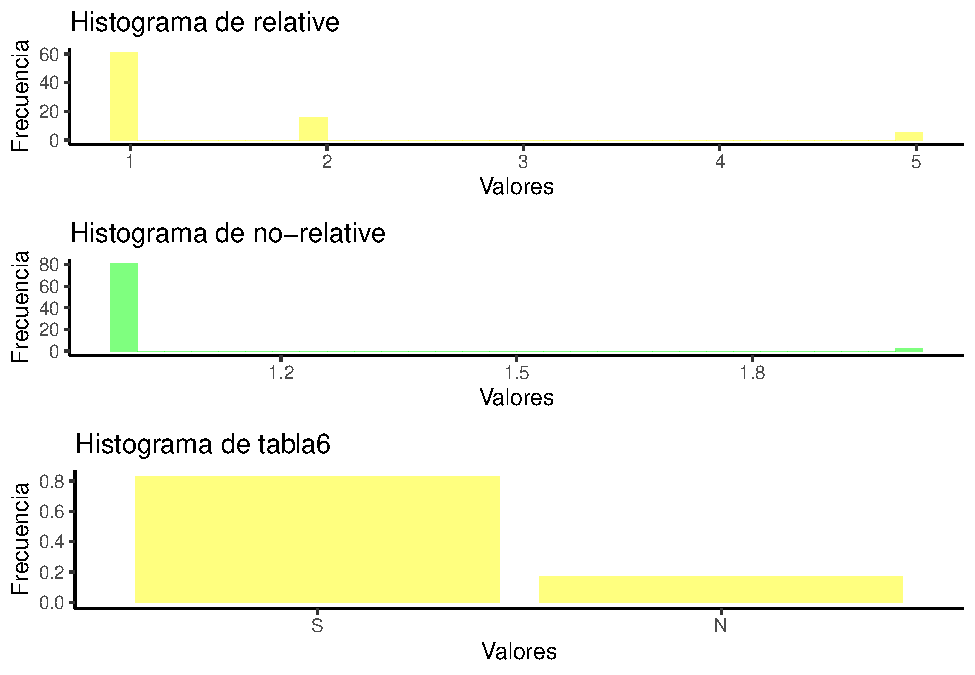
\includegraphics{Practica_2_files/figure-latex/histobarras-1.pdf}

PREGUNTA 2.3

\begin{Shaded}
\begin{Highlighting}[]
\CommentTok{\# Crea datos}
\NormalTok{relative }\OtherTok{\textless{}{-}}\NormalTok{ tabla2}
\NormalTok{no\_relative }\OtherTok{\textless{}{-}}\NormalTok{ tabla3}

\CommentTok{\# Genera 1er histograma}
\NormalTok{p1 }\OtherTok{\textless{}{-}} \FunctionTok{ggplot}\NormalTok{(}\FunctionTok{data.frame}\NormalTok{(}\AttributeTok{x=}\NormalTok{relative), }\FunctionTok{aes}\NormalTok{(}\AttributeTok{x=}\NormalTok{x)) }\SpecialCharTok{+} 
  \FunctionTok{geom\_histogram}\NormalTok{(}\FunctionTok{aes}\NormalTok{(}\AttributeTok{y=}\NormalTok{..count..), }\AttributeTok{fill=}\StringTok{"yellow"}\NormalTok{, }\AttributeTok{alpha=}\FloatTok{0.5}\NormalTok{) }\SpecialCharTok{+}
  \FunctionTok{labs}\NormalTok{(}\AttributeTok{title=}\StringTok{"Histograma de relative"}\NormalTok{, }\AttributeTok{x=}\StringTok{"Valores"}\NormalTok{, }\AttributeTok{y=}\StringTok{"Frecuencia"}\NormalTok{) }

\CommentTok{\# Genera 2do histograma}
\NormalTok{p2 }\OtherTok{\textless{}{-}} \FunctionTok{ggplot}\NormalTok{(}\FunctionTok{data.frame}\NormalTok{(}\AttributeTok{x=}\NormalTok{no\_relative), }\FunctionTok{aes}\NormalTok{(}\AttributeTok{x=}\NormalTok{x)) }\SpecialCharTok{+} 
  \FunctionTok{geom\_histogram}\NormalTok{(}\FunctionTok{aes}\NormalTok{(}\AttributeTok{y=}\NormalTok{..count..), }\AttributeTok{fill=}\StringTok{"green"}\NormalTok{, }\AttributeTok{alpha=}\FloatTok{0.5}\NormalTok{) }\SpecialCharTok{+}
  \FunctionTok{labs}\NormalTok{(}\AttributeTok{title=}\StringTok{"Histograma de no{-}relative"}\NormalTok{, }\AttributeTok{x=}\StringTok{"Valores"}\NormalTok{, }\AttributeTok{y=}\StringTok{"Frecuencia"}\NormalTok{)}

\CommentTok{\# Genera 2do histograma}
\NormalTok{factor\_tabla6 }\OtherTok{\textless{}{-}} \FunctionTok{factor}\NormalTok{(tabla6, }\AttributeTok{levels =} \FunctionTok{c}\NormalTok{(}\StringTok{"S"}\NormalTok{, }\StringTok{"N"}\NormalTok{))}

\CommentTok{\# Data frame columna "x"}
\NormalTok{data }\OtherTok{\textless{}{-}} \FunctionTok{data.frame}\NormalTok{(}\AttributeTok{x =}\NormalTok{ factor\_tabla6)}

\CommentTok{\# Genera el histograma}
\NormalTok{p3 }\OtherTok{\textless{}{-}} \FunctionTok{ggplot}\NormalTok{(data, }\FunctionTok{aes}\NormalTok{(}\AttributeTok{x =}\NormalTok{ x)) }\SpecialCharTok{+} 
  \FunctionTok{geom\_bar}\NormalTok{(}\FunctionTok{aes}\NormalTok{(}\AttributeTok{y=}\NormalTok{..count..}\SpecialCharTok{/}\FunctionTok{sum}\NormalTok{(..count..)), }\AttributeTok{fill=}\StringTok{"yellow"}\NormalTok{, }\AttributeTok{alpha=}\FloatTok{0.5}\NormalTok{, }\AttributeTok{stat =} \StringTok{"count"}\NormalTok{) }\SpecialCharTok{+}
  \FunctionTok{labs}\NormalTok{(}\AttributeTok{title=}\StringTok{"Histograma de tabla6"}\NormalTok{, }\AttributeTok{x=}\StringTok{"Valores"}\NormalTok{, }\AttributeTok{y=}\StringTok{"Frecuencia"}\NormalTok{)}

\NormalTok{p4 }\OtherTok{\textless{}{-}} \FunctionTok{ggplot}\NormalTok{(}\FunctionTok{data.frame}\NormalTok{(}\AttributeTok{x=}\NormalTok{tabla7), }\FunctionTok{aes}\NormalTok{(}\AttributeTok{x=} \StringTok{""}\NormalTok{, }\AttributeTok{fill =}\NormalTok{ x)) }\SpecialCharTok{+} 
  \FunctionTok{geom\_bar}\NormalTok{(}\AttributeTok{width =} \DecValTok{1}\NormalTok{) }\SpecialCharTok{+} \FunctionTok{coord\_polar}\NormalTok{(}\AttributeTok{theta =} \StringTok{"y"}\NormalTok{) }\SpecialCharTok{+}
  \FunctionTok{labs}\NormalTok{(}\AttributeTok{title=}\StringTok{"status code"}\NormalTok{)}

\CommentTok{\# Ordena gráficos}
\FunctionTok{theme\_set}\NormalTok{(}\FunctionTok{theme\_classic}\NormalTok{())}

\CommentTok{\# Reordena 2 filas, 1 columna }
\FunctionTok{ggarrange}\NormalTok{(p1, p2, p3, p4, }\AttributeTok{ncol=}\DecValTok{1}\NormalTok{, }\AttributeTok{heights=}\FunctionTok{c}\NormalTok{(}\DecValTok{1}\NormalTok{,}\DecValTok{1}\NormalTok{,}\DecValTok{1}\NormalTok{,}\FloatTok{1.2}\NormalTok{))}
\end{Highlighting}
\end{Shaded}

\begin{verbatim}
## `stat_bin()` using `bins = 30`. Pick better value with `binwidth`.
## `stat_bin()` using `bins = 30`. Pick better value with `binwidth`.
\end{verbatim}

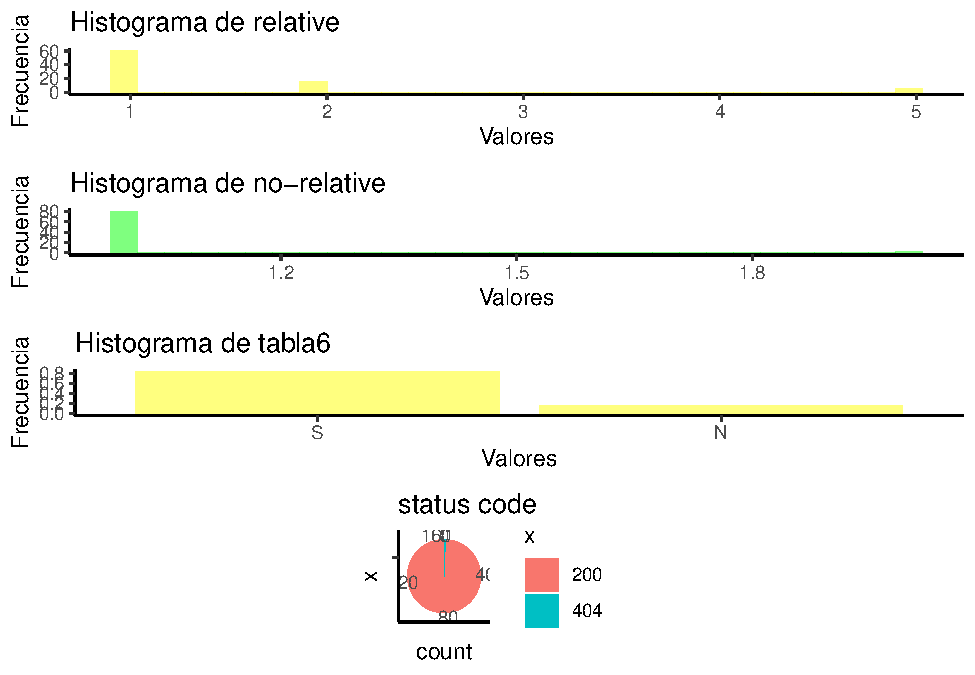
\includegraphics{Practica_2_files/figure-latex/chart_graphic-1.pdf}

\end{document}
